\clearpage
\subsubsection{Break} % (fold)
\label{sub:break}

The break statement is used to jump out of the current loop, in effect terminating the loop early. This is useful for ending the current loop, skipping all future cycles.

\begin{figure}[h]
   \centering
   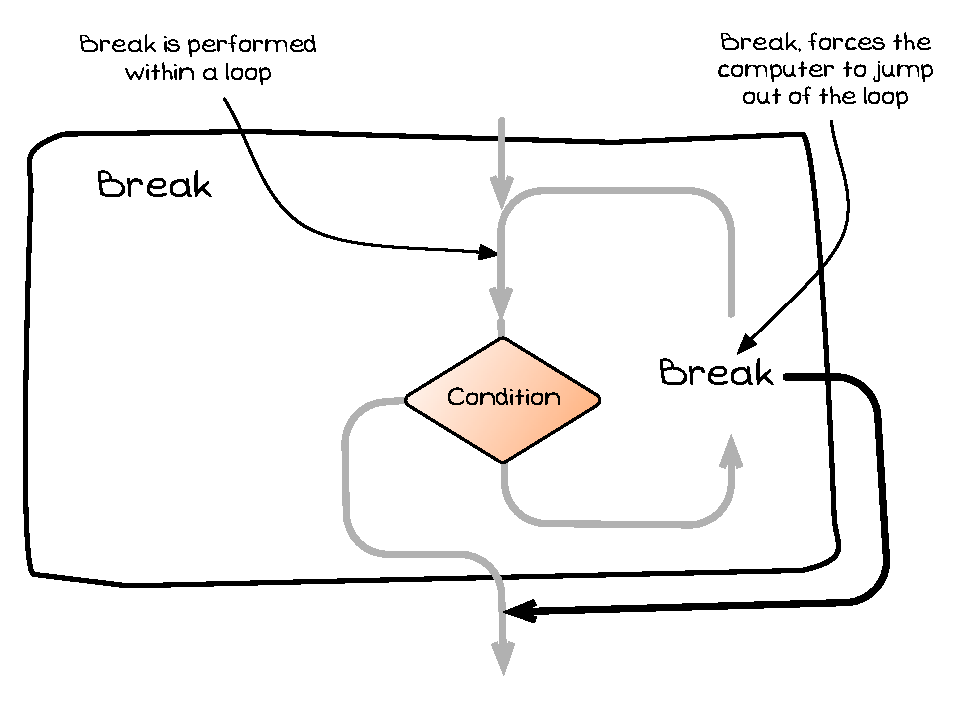
\includegraphics[width=\textwidth]{./topics/control-flow/diagrams/Break} 
   \caption{The Break Statement allows you to end a loop early}
   \label{fig:break}
\end{figure}

\mynote{
\begin{itemize}
  \item The break statement is an \textbf{action}, allowing you to jump to the end of the current loop.
  \item The break statement should be coded within an \nameref{sub:branching} statement that checks if the loop should terminate early.
\end{itemize}
}


% subsection break (end)